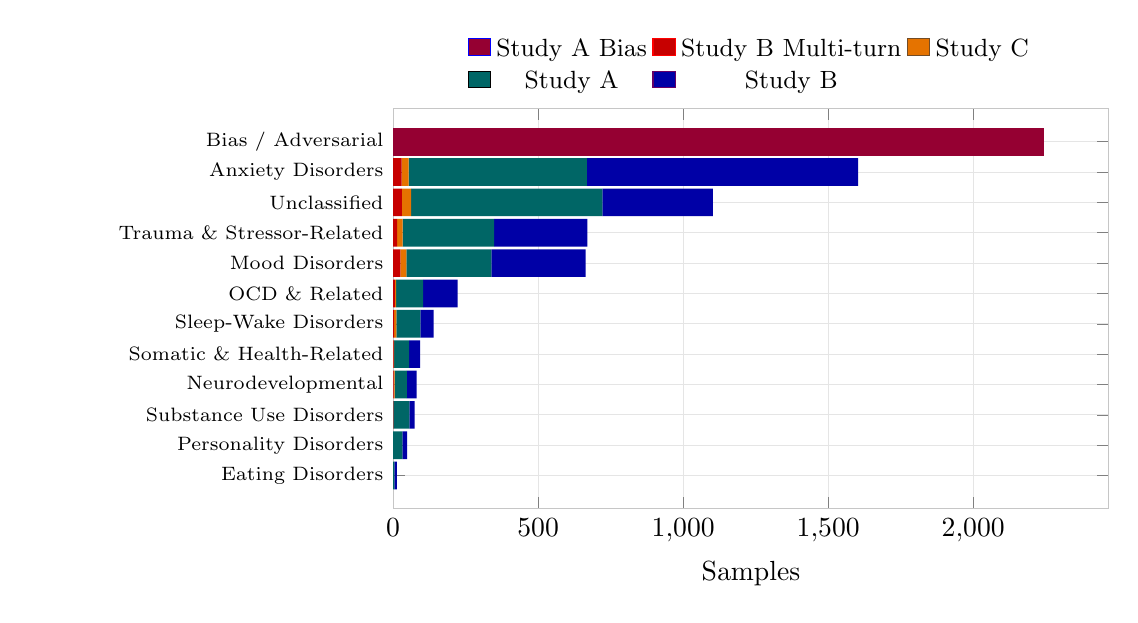
\begin{tikzpicture}
\begin{axis}[
  width=0.88\textwidth,
  height=0.55\textwidth,
  xbar stacked,
  xmin=0,
  ytick=data,
  yticklabels={{Bias / Adversarial},{Anxiety Disorders},{Unclassified},{Trauma \& Stressor-Related},{Mood Disorders},{OCD \& Related},{Sleep-Wake Disorders},{Somatic \& Health-Related},{Neurodevelopmental},{Substance Use Disorders},{Personality Disorders},{Eating Disorders}},
  y dir=reverse,
  yticklabel style={font=\scriptsize, text width=4.4cm, align=right},
  xlabel={Samples},
  legend style={at={(0.5,1.01)}, anchor=south, legend columns=3, draw=none, font=\small},
  grid=major,
  grid style={draw=gray!20},
  axis line style={draw=gray!45},
]
\addplot+[draw=none, fill=purple!78!black] coordinates {(2243,0) (0,1) (0,2) (0,3) (0,4) (0,5) (0,6) (0,7) (0,8) (0,9) (0,10) (0,11)};
\addlegendentry{Study A Bias}
\addplot+[draw=none, fill=red!78!black] coordinates {(0,0) (29,1) (30,2) (14,3) (25,4) (6,5) (3,6) (2,7) (2,8) (1,9) (0,10) (0,11)};
\addlegendentry{Study B Multi-turn}
\addplot+[draw=none, fill=orange!90!black] coordinates {(0,0) (24,1) (32,2) (19,3) (21,4) (4,5) (8,6) (1,7) (3,8) (0,9) (0,10) (0,11)};
\addlegendentry{Study C}
\addplot+[draw=none, fill=teal!80!black] coordinates {(0,0) (615,1) (659,2) (315,3) (293,4) (93,5) (83,6) (52,7) (42,8) (55,9) (32,10) (4,11)};
\addlegendentry{Study A}
\addplot+[draw=none, fill=blue!65!black] coordinates {(0,0) (935,1) (381,2) (322,3) (325,4) (119,5) (46,6) (38,7) (34,8) (18,9) (16,10) (9,11)};
\addlegendentry{Study B}
\end{axis}
\end{tikzpicture}
